% !TeX spellcheck = sk_SK

\section{Analýza problému}


\subsection{Petriflow}
Carl Adam Petri založil koncept Petriho sietí v roku 1962 vo svojej dizertačnej práci - Komunikácia s Automatmi - na Technickej Univerzite v Darmstadte. Ďalším výskumom sa z pôvodného konceptu ktorý bol určený na modelovanie analýzu komunikačných systémov vyvinul nástroj, ktorý sa používa naprieč mnohými oblasťami najmä na modelovanie paralelných a distribuovaných systémov.

Formalizmus Petriflow je rozšírenie Petriho sietí, ktoré bolo navrhnuté na modelovanie komplexných biznis procesov. Je vyvíjaný spoločnosťou Netgrif na základe dlhodobých skúseností s klientami, ktorý pomocou tohto formalizmu modelujú svoje biznis procesy, ktoré sú následne zavedené do používania.

Formalizmus Petriflow rozširuje Petriho siete o ďalšie komponenty. Ako základ berie Petriho siete obohatené reset, inihibitor a read hrany. Aby sa dali modelovať moderné biznis procesy pridáva Petriflow do tohto modelu roly, dátové polia a akcie.

Roly definujú kto je oprávnený spúšťať rôzne prechody.

Dátové polia definujú štruktúru dát ktoré každá inštancia procesu obsahuje počas svojho behu.

Akcie definujú vzťahy a interakcie medzi jednotlivými dátovými poľami a prechodmi.

V klasických Petriho sieťach je spustenie prechodu vždy atomická operácia. Petriflow obsahuje dva typy prechodov. Udalostné prechody, ktoré sú rovnako  ako v klasických PN sieťach atomické, avšak vždy ich spúšťa nejaká osoba(používateľ) v systéme. Druhý typ prechodu je úloha. Úlohu môžeme vnímať ako podsieť na obrázku \ref{task}. Na začiatku je úloha nepridelená, ako prvý krok je potrebné ju niekomu (aj sebe) prideliť. Následne môže toto pridelenie zrušiť, prideliť inej osobe, alebo úlohu dokončiť. My sa ďalej budeme zaoberať ľen úlohami.

Keďže každá úloha je samostatná sieť so štyrmi prechodmi, musíme pre každú úlohu zadafinovať roly pre všetky štyri operácie úlohy.

\begin{figure}[!htbp]
	\centering
	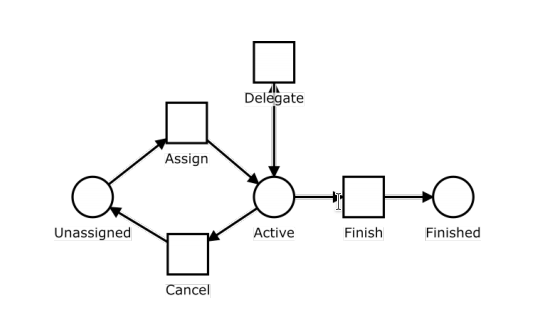
\includegraphics[width=6cm]{img/task_transition.png}
	\caption{Úloha}
	\label{task}
\end{figure}

\subsection{Aplikačné rozhranie}
Majme procesne orientovaný systém ktorý implementuje procesy, popísane v Petriflow. S takýmto systémom používatelia interagujú iba presne popísaným spôsobom a to spúšťaním prechodov ktoré majú podľa svojich rolí oprávnenie spúšťať (delegovať, dokončiť,... ). Pri dokončení úlohy (prechodu) musí používateľ poskytnúť dáta popísané v dátových poliach.

Keďže formalizmus Petriflow je schopný takýmto spôsobom popísať všetky interakcie používateľa so systémom je možné na jeho základe vygenerovať aj aplikačné rozhranie. Toto rozhranie sprístupní systém mimo jeho domény, zaručí autorizáciu podľa rolí, poskytne dokumentáciu o svojej štruktúre(a tým pádom aj štruktúre procesu) a zabezpečí validáciu dát, ktoré do systému používateľ odošle.

Ak by rozhranie držalo informáciu o značkovaní, a teda spustiteľnosti prechodov, mohol by nasať stav kedy aplikačné rozhranie je v stave, ktorý naznačuje, že prechod sa nedá spustiť no procesný server už je v stave, kedy je prechod spustiteľný. Kvôli udržaniu konzistencie dát a predídeniu race conditions nemôže aplikačné rozhranie držať informáciu o značkovaní a teda ani spustiteľnosti prechodu.

Aktuálna verzia Petriflow poskytuje relatívne granulárne informácie o autorizácií na vykonávanie akcií pomocou rolí, neobsahuje však informáciu o používateľoch ani o tom ktorý používateľ má pridelené aké roly. Na implementáciu funkčného aplikačného rozhrania teda bude nutné dorobiť systém ktorý túto informáciu bude obsahovať.

%TODO obrazok viacero PN -> viac endpointov API - point very cloudy

\section{Špecifikácia}

V tejto kapitole najprv stručne opíšeme hlavnú funkcionalitu navrhovanej aplikácie, potom zadefinujeme funkcionálne a nefunkcionálne požiadavky na aplikáciu.

Softvér, ktorý sme sa rozhodli implementovať bude slúžiť ako rozhranie medzi procesným serverom a internetom. Bude umožňovať klientovi pripojiť sa na procesný server cez internet, autentifikovať sa, získať informácie o dátach v prechodoch petriho siete a bude umožňovať modifikovať stav siete (procesu) spúšťaním prechodov.

\subsection{Funkcionálne požiadavky}

\begin{enumerate}
	\item Rozhranie bude umožňovať administrátorovi registrovať používateľov a priraďovať im roly
	\item Umožní administrátorovi za behu pridať nové koncové body a meniť, alebo vymazať aktuálne nasadené koncové body
	\item Umožní prihlásenie používateľa pomocou štandardného autentifikačného protokolu.
	\item Autentifikovaným používateľom umožní prístup k dátam z tých prechodov ktoré majú právo čítať podľa ich roly.
	\item Autentifikovaným používateľom umožní spúšťať prechody ktoré majú právo spúšťať podľa ich roly.
	\item Pri spúšťaní prechodu prebehne validácia vstupných dát. V prípade nevalidných alebo nekompletných dát nepovolí spustenie prechodu.
	\item Rozhranie poskytne online dokumentáciu prechodov v sieti, táto dokumentácia bude zahŕňať URL prechodu, potrebné dátové polia na spustenie prechodu a roly, ktoré sú oprávnené prechody spúšťať.
	\item Rozhranie poskytne aplikačné rozhranie viacerým sieťam s rôznou štruktúrou. A viacerým inštanciám týchto sietí.
\end{enumerate}

\subsection{Nefunkcionálne požiadavky}
\begin{enumerate}
	\item Rozhranie bude škálovateľné
	\item Rozhranie bude zabezpečené štandardnými bezpečnostnými prvkami
	\item Rozhranie bude bežať na serveri poskytnutom Fakultou Elektrotechniky a Informatiky na Slovenskej Technickej Univerzite v Bratislave.
\end{enumerate}

\section{Návrh}

\subsection{Prípady použitia}
Zo špecifikácie vyplývajú nasledovné interakcie používateľa s naším systémom.

\subsubsection{Registrácia modelu}
Prvý prípad použitia je registrácia modelu. Aktér ktorý môže registrovať modely je len administrátor. Pri tejto akcií administrátor poskytne nášmu systému informácie o štruktúre procesu vo formáte petriflow, zoznam používateľov im prislúchajúcich rolí v \acrshort{xml} a unikátny identifikátor siete.

Pokiaľ chce administrátor upraviť nasadený proces spustí proces registrácie nanovo s upravenými údajmi o sieti, používateľoch a rolách.

Administrátor taktiež môže sieť vymazať.

\subsubsection{Získanie informácie o prechode}
Keď už sú sieť aj používatelia úspešne zaregistrovaný, si môžu používatelia, vyžiadať informácie o prechode. Tieto informácie budú poskytnuté len používateľovi s rolou oprávnenou na čítanie dát z daného prechodu.

\subsubsection{Vykonanie akcie na prechode}
Používatelia s príslušnými rolami môžu taktiež vykonávať akcie na prechodoch. Tieto akcie vyplývajú z definície petriflow a patrí medzi ne assign, delegate, cancel, a finish. Na každú z týchto akcií potrebuje používateľ mať opávnenie (rolu, ktorá je oprávnená vykonávať túto akciu), a každá z nich vyžaduje iné vstupné dáta.

\subsubsection{Autentifikácia}
Z požiadavky na bezpečnosť aplikácie vyplýva ešte prípad použitia, kedy sa používateľ autentifikuje, aby nadobudol identitu rozpoznanú našim systémom a boli mu pridelené roly.

\subsection{Štruktúra aplikačného rozhrania}
Náš systém musí prihláseným používateľom poskytnúť možnosť získavať informácie o stave prechodov a na prechodoch vykonávať rôzne akcie. Musí pracovať s rôznymi štruktúrami a viacerými inštanciami týchto procesov. Preto navrhujeme štruktúru aplikačného rozhrania nasledovne.

URL ktoré bude klient volať sa budú skladať zo štyroch častí.
\begin{enumerate}
	\item identifikátor siete
    \item číslo inštancie procesu
	\item identifikátor prechodu
	\item vykonávanú operáciu
\end{enumerate}
Príklad URL ciest pre jednu úlohu môžeme vidieť na ukážke \ref{alg:urls_example}

\begin{lstlisting}[ caption={Ukážka URL ciest k úlohe},label={alg:urls_example}]
GET:
/ExampleNet/0/t1

POST:
/ExampleNet/0/t1/assign
/ExampleNet/0/t1/delegate
/ExampleNet/0/t1/cancel
/ExampleNet/0/t1/finish
\end{lstlisting}

Prvá cesta má HTTP metódu GET a predstavuje operáciu čítania aktuálnych dát v úlohe na danej inštancií procesu. Ostatné operácie majú metódu POST a reprezentujú dané operácie na inštancii úlohy.

Okrem generovaných ciest pre procesy potrebujeme vyhradiť ešte cesty pre administrátora na obsluhu rozhrania. bude to cesta "/" s metódami POST a DELETE, určené pridávanie a vymazávanie procesov.

\subsection{Architektúra}
Aby sme splnili požiadavku na jednoduché škálovanie aplikácie a pre sprehľadnenie architektúry zvolili sme si architektúru mikroservisov. Táto architektúra pozostáva z viacerých oddelených častí, každá z týchto častí má svoju jasne definovanú funkciu. Takéto mikroservisy sú jednoducho testovateľné, dajú sa nasadzovať postupne a nezávisle od seba a softvér navrhnutý v tejto architektúre býva spravidla robustný a vysoko škálovateľný.

Softvér sa bude skladať z troch hlavných služieb: generátor, relay bod a autentifikačná služba.

\begin{itemize}
    \item Generator je služba, ktorá bude registrovať a zostavovať koncové body. Je to služba, na ktorú sa pripojí administrátor, zadá štruktúru siete a zoznam používateľov a rolí. Táto služba následne zaregistruje používateľov a ich roly, vygeneruje kód pre službu relay a túto službu spustí.
	\item Relay je služba, ktorá obsahuje vygenerovaný kód koncových bodov. Táto služba bude poskytovať dokumentáciu dostupných koncových bodov. bude poskytovať samotné koncové body a pri zavolaní koncového bodu sa bude starať o validáciu prijatých dát.
	\item Autentifikačná služba sa stará o autentifikáciu používateľov a prideľovanie rolí používateľom
	\item Gateway služba poskytuje rozhranie medzi internetom a našou doménou. Vonkajšiemu svetu prezentuje len služby ktoré majú byť dostupné z internetu. Zároveň poskytuje funkcionalitu load balancera.
    \item Service discovery je služba ktorá monitoruje stav všetkých ostatných kontajnerov a vie poskytnúť informácie o stave systému, toto je potrebné na správnu operáciu load balancera.
\end{itemize}

\begin{figure}[!htbp]
	\centering
	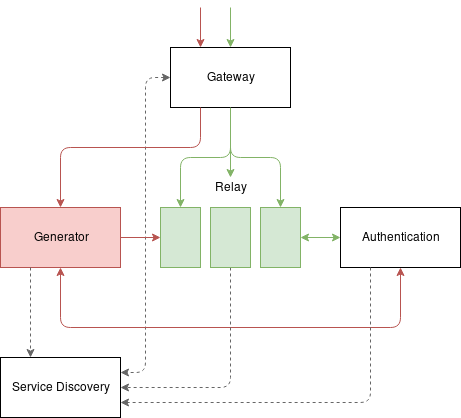
\includegraphics[width=10cm]{img/architecture.png}
	\caption{Architektúra rozhrania}
	\label{architecture}
\end{figure}

\subsection{Bezpečnosť}

Autentifikáciu v našej aplikácií budeme riešiť pomocou štandardnej knižnice, ktorá poskytuje \acrshort{oauth}. Táto služba bude bežať v samostatnom kontajnery a prístup do nej bude len pomocou protokolu \acrshort{oauth} na overovanie klientov a prostredníctvom interného volania na registráciu používateľov.

Ochrana pred neoprávneným prístupom bude ďalej realizovaná pomocou služby gateway. Táto služba bude jediný bod ako sa dá pristúpiť do našej domény z internetu. Služba bude povoľovať len dotazy ktoré špecifikujeme. Ochrana proti neopevnenému prístupu bude taktiež realizovaná na vrstve operačného systému pomocou firewallu.

Ochrana proti \acrshort{dos} útokom bude taktiež realizovaná pomocou gateway služby. Táto služba bude slúžiť ako load balancer, a rovnomerne rozdeľovať dotazy medzi inštancie relay servisu tak, aby boli rovnomerne vyťažené.

\subsection{Operácia systému}
Na diagrame \ref{api_operation} vidíme vo vrchnej časti proces prihasenia používateľa a v dolnej časti vykonanie dopytu na procesný server.

Počas procesu prihlásenia používateľ najprv odošle dopyt na prihlásenie, gateway ho presmeruje na autorizačný servis a ten mu následne vráti autorizačný token.

Proces dopytu na procesný server je zložitejší. Najprv klient pošle dopyt na náš systém, gateway ho nasmeruje na relay servis, ktorý si podľa autorizačného tokenu vypýta od auth servisu profil používateľa, pokiaľ má rolu potrebnú na spustenie prechodu a dotaz je validný, odošle relay dopyt ďalej na procesný server. Odpoveď z procesného servera sa následne propaguje spať ku klientovi.

\begin{figure}[!htbp]
	\centering
	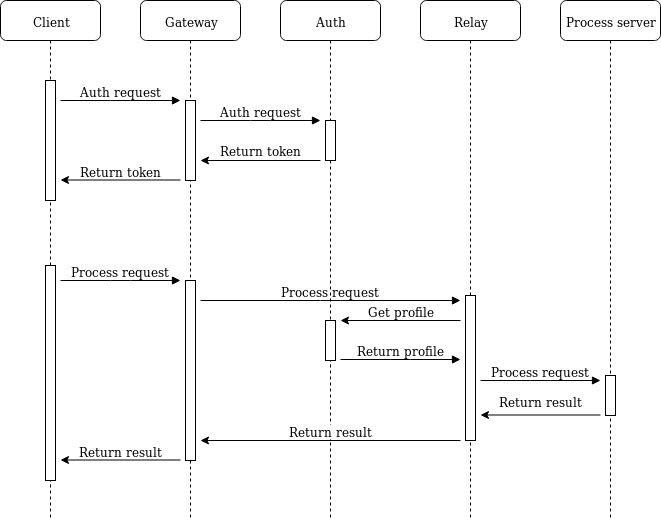
\includegraphics[width=10cm]{img/api_operation.png}
	\caption{Operácia rozhrania}
	\label{api_operation}
\end{figure}

Proces zmeny rozhrania ako môžeme vidieť na diagrame \ref{change_operation}.
Po tom, čo náš systém prijme požiadavku na zmenu rozhrania, najprv vyčistí prostredie, a stiahne najnovšiu verziu relay servisu. Následne vygeneruje kód koncových bodov, a zostavovanie tohto kódu. Ak prebehlo zostavovanie kódu v poriadku, a teda vygenerovaný ód je validný, odošleme pokyn na zastavenie starého rozhrania a paralelne spustíme proces registrácie nových používateľov a spustenie nového rozhrania. Naše rozhranie teda bude mať výpadok, len v období medzi vypnutím starej a zapnutím novej inštancie relay servisu.

\begin{figure}[!htbp]
	\centering
	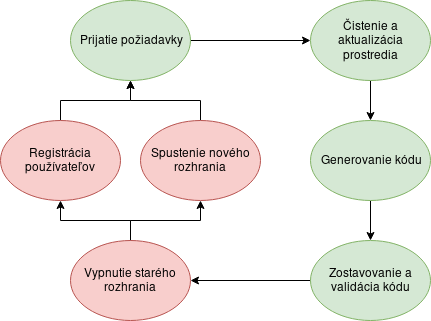
\includegraphics[width=10cm]{img/change_operation.png}
	\caption{Proces zmeny rozhrania}
	\label{change_operation}
\end{figure}

\section{Implementácia}
V tejto kapitole najprv predstavíme technológie ktoré sme použili pri implementácií nášho systému, následne predstavíme jednotlivé kontajnery nášho distribuovaného.

\subsection{Použité technológie}

\subsubsection{Kotlin}
Kotlin je relatívne nový programovací jazyk, projekt Kotlin bol po prvý krát zverejnený v roku 2011 spoločnosťou JetBrains(Andrey Breslav). Bol vyvinutý ako moderný staticky typovaný jazyk, ktorý podporuje rýchlu kompiláciu do javy. V roku 2017 ohlásil Google podporu pre Kotlin v operačnom systéme Android. V rovnakom roku ohlásil Pivotal Software oficiálnu podporu pre Kotlin vo verzii 5.0 ich frameworku Spring.

Kotlin sa dá buď transpilovať do jazyka Java, alebo JavaScript, alebo sa dá kompilovať priamo do spustiteľného binárneho súboru pe všetky bežné operačné systémy (Linux, Windows, Android, iOS).

Jazyk bol navrhnutý tak, aby bol čo najviac čitateľný, čo najviac sa vyhol potrebe písať zbytočný, alebo duplicitný kód a aby sa čo najviac vyhol chybám pri behu systému, a odchytal chyby už pri kompilácií. Na nasledujúcich príkladoch si ukážeme akými spôsobmi dosiahli tvorcovia tohto jazyku tieto ciele. 

V jazyku Kotlin sa deklarujú premenné pomocou kľúčových slov val alebo var, takto deklarujeme buď konštanty, alebo premenné. samotný typ premennej je vo väčšine prípadov odvodený z hodnoty ktorú premennej pridelíme. V prípade, že zadefinujeme premennú pomocou var a nemutujeme jej obsah, kompilátor hlási varovanie, že premenná môže byť zmenená na konštantu. Tento prístup však funguje len pri primitívnych dátových typoch. Pri kontajneroch sa uplatňuje rovnaký princíp použitím imutabilných dátových štruktúr list, map, a ďalšie. Ak chceme zadeklarovať list ktorého obsah plánujeme meniť musíme použiť typ mutableList. 

Ďalšie vylepšenie typového systému prichádza implementáciou nulovateľných typov. Tento princíp obmedzuje potrebu používania try cathc blokov a na miesto toho ich nahradzuje nulovateľnými typmi. Ak pracujeme s funkciou, ktorá nemusí vždy vrátiť dáta, jej vstupný typ bude nulovateľný. Pri práci s takýmito nulovateľnými typmi nám kompilátor núti ošetriť prípady, kedy premenná obsahuje null. Na ukážke kódu \ref{alg:kt_null} vidíme, príklad funkcie, ktorá vracia nulovateľný String?. Ak sa pokúsime pristúpiť k parametru length tejto premennej pred tým ako ošetríme nulový prípad, kompilátor vyhlási kompilačnú chybu a nedovolí nám kód skompilovať. Ak by sme tento prípad neošetrili v Jave by došlo k chybe až pri behu programu. 

Ak korektne ošetríme nulový prípad kompilátor zmení ty premenenej na nenulovatľný a dovolí nám ďalej pracovať s premennou, lebo už je zaučené, že nenastane chyba pri prístupe k dátam. 


\begin{lstlisting}[ caption={Ukážka funkcie typov v jazyku Kotlin},label={alg:kt_null},language=Kotlin]
// vráti null alebo String
fun maybeGetString():String?

// typ String? - môže obsahovať null, nieje nutné typ explicitne definovať je inferovaný z výstupného typu finkcie
val variable = maybeGetString()

// nastane chyba pri kompilácií, lebo nieje ošetrený prípad, kedy je valiable null
print(variable.length)

if(isNullOrEmpty(variable){
	variable = "placeholder"
}

// nenastane chyba pri kompilácií, lebo bol ošetrný nulový priípad
// typ String - už nemôže byť null, iba string
print(variable.length)
\end{lstlisting}


Ďalšie zlepšenie jazyka ktoré je veľmi užitočné pri práci s frameworkom Spring sú dátové triedy. Ak by sme v Jave chceli vytvoriť jednoduchú triedu, ktorá len drží dáta, musíme zadeklarovať triedu, jej konštruktor, dátové polia, a funkcie na nastavovanie a čítanie polí. v jazyku Kolin vieme zadeklarovať dátovú triedu pomocou jednoriadkového príkazu. Na ukážke kódu \ref{kt_dataclass} vidíme príklad dátovej triedy Person s povinnými prvými dvomi poľami firstName a lastName a nepovinnými poľami age a height. Pole firstName je konštantné, preto sa nebude dať meniť nie je nutné vynechať implementáciu nastavovacej funkcie ako v Jave. Polia age a height sú nepovinné.  
 
V jazyku Kotlin je implementovaný aj princíp pomenovaných argumentov. To znamená, že konštruktor našej dátovej triedy Person môžeme zavolať s ľubovoľnou kombináciou nepovinných argumentov. 

\begin{lstlisting}[ caption={Ukážka dátových tried a pomenovaných argumentov v jazyku Kotlin},label={alg:kt_dataclass},language=Kotlin]
	data class Person(
		val firstName: String,
		var lastName: String,
		var age?: Int,
		var height:? Int)

  val p1 = Person("Jozef", "Mrkva", height=180)		
	\end{lstlisting}



My sme zvolili jazyk Kotlin pre náš projekt hlavne kvôli vylepšeniam v systéme typovania a zmenšenému boilerplatu. Ďalej nám využitie tohto jazyka umožnila bezproblémová integrácia s frameworkom Stping a ostatnými knižnicami v jazyku Java.	

\subsubsection{Gradle}
Gradle je voľne šíriteľný nástroj na automatizáciu zostavovania softvéru. Je stavaný na to aby bol schopný zostaviť takmer ľubovoľný program. Podporuje jazyky ako Java, C++ Python, a mnoho ďalších. V našom projekte sa gradle použijeme na manažment závislostí, kompiláciu kódu a spustenie samotného skompilovaného programu. Konfigurácia nástroja prebieha pomocou konfiguračného súboru napísaného v jazyku Groovy, tieto konfiguračné  súbory sa v našom prípade použitia ukázali ako veľmi prehľadné a ľahké na použitie. Gradle taktiež používa pokročilú techniku memoizácie procesu zostavovania softvéru takže jeho výkon je pri opakovanej kompilácií vyšší.

\subsubsection{Spring}
Spring je jeden z najpoužívanejších frameworkov využívaných Java developermi. Framework je voľne šíriteľný a udržiavaný spoločnosťou Pivotal Software, Inc.
%TODO SPPRING

Všetky Spring Boot kontajnery sme inštalovali pomocou Spring initializr \cite{initializr}

tento nástroj vygeneruje zip súbor so založeným projektom vo frameworku Spring Boot. Pri vytváraní projektu je možné si vybrať Jazyk v ktorom bude projekt založený a nástroj ktorý bude projekt zostavovať % --

\subsubsection{Spring cloud}

Spring Cloud je framework, ktorý obsahuje bohatú sadu nástrojov na vytváranie mikroservisov a cloudových riešení. Medzi nástroje Spring Clopudu patí:

\begin{itemize}
	\item Cloud config - nástroj na distribúciu konfiguračných súborov medzi kontajnermi mikroservisov
	\item Service discovery - nástroj na registráciu a monitorovanie mikroservisov
    \item Gateway - Nástroj na smerovanie a load balancing v rámci mikroservisov
	\item Cloud Authentication - Nástroj na riešenie komplexnej autentizácie a autorizácie v rámci

\end{itemize}
%TODO Spring Cloud

\subsubsection{Git}
Git je najpoužívanejší nástroj na kontrolu revízií na svete. Bol vytvorený Linusom Torvaldsom v roku 2005 na kontrolu revízií pri vývoji jadra Linuxu. A rovnako ako Linux bol zverejnený na voľné používanie. V našom projekte sme použili git na kontrolu revízií samotného kódu našej aplikácie. Zároveň sme využili Java knižnicu JGit \cite{jgit}, čo je implementácia gitu v jave. Bola vyvinula a je ďalej udržiavaná spoločnosťou Eclipse Foundation, Inc.

\subsubsection{Insomnia}
Insomnia \cite{insomnia} je voľne šíriteľný softvér vyvíjaný spoločnosťou Floating Keyboard Software Inc. Je určený na testovanie REST a GraphQL služieb. Je to alternatíva ku známemu programu Postman. Je postavený na platforme Electron s použitím knižnice React. Insomnia nám dovolí vytvoriť a uložiť viacero testovacích dopytov, ktoré môžeme neskôr spustiť a overiť ich správne fungovanie. Insomnia taktiež podporuje autentifikačný protokol OAuth2. Okrem štandardných HTTP volaní podporuje aj čoraz viac populárny protokol GraphQL

\subsection{Generator service}
Tento servis je základný stavebný kameň nášho rozhrania, jeho úlohou je na základe vstupu v podobe procesného modelu vo formáte Petriflow vygenerovať a spustiť inštancie relay service, ktorý bude prijímať samotné požiadavky od klienta. Základná operácia vygenerovania koncového dobu má nasledovné kroky:
prijatie požiadavky,
čítanie súborov Petriflow a súborov s používateľmi,
registrácia používateľov,
príprava repozitára,
generovanie kódu
a kompilácia a spustenie relay.

\subsubsection{Prijatie požiadavky}
Pre funkciu pridania požiadavky je v našom systéme vyhradená základná URL "/[POST]", na tejto URL je funkcia, ktorá berie ako parametre súbor s procesným modelom, súbor s používateľmi a unikátny identifikátor siete. Súbor s modelom je v štandardnom formáte Petriflow. Súbor s používateľmi je vo formáte \acrshort{xml} so štruktúrou popísanou \acrshort{xsd} súborom v prílohe \ref{att:xsd}. Tento XSD súbor je poskytnutý aj v rámci dokumentácie v \acrshort{openapi}. Na príklade súboru v ukážke kódu \ref{alg:example_users} môžeme vidieť že súbor obsahuje zoznam používateľov s menom, heslom a zoznamom ich rolí.

\begin{lstlisting}[float, caption={Príklad súboru s používateľmi},label={alg:example_users},language=XML]
<?xml version="1.0" encoding="UTF-8"?>
<document xmlns:xsi="http://www.w3.org/2001/XMLSchema-instance" xsi:noNamespaceSchemaLocation="./users_schema.xsd">
	<user name="admin" password="SecureAdminPass">
		<role id="client"/>
		<role id="bureau_agent"/>
		<role id="loan_officer"/>
		<role id="underwriter"/>
		<role id="property_appraiser"/>
		<role id="account_clerk"/>
	</user>
	<user name="user1" password="SecureUser1Pass">
		<role id="bureau_agent"/>
		<role id="underwriter"/>
		<role id="account_clerk"/>
	</user>
	<user name="user2" password="SecureUser2Pass">
		<role id="client"/>
		<role id="loan_officer"/>
		<role id="property_appraiser"/>
	</user>
</document>
\end{lstlisting}

Funkciu registrácie môže spustiť iba administrátor systému(Viac v časti Auth Service \ref{section_auth}).

Tieto súbory sa uložia do priečinka na servery s názvom Net[ID siete] a Users[ID siete]. V prípade, že už existujú súbory s rovnakým ID tieto súbory sa prepíšu a tým zaručujeme funkcionalitu zmeny siete.

Ukladanie súboru s heslami v textovej forme je v produkčnej aplikácií neprípustné, preto pred uložením vytvoríme hash hesla štandardným spôsobom kompatibilným so Spring Security.

Okrem požiadavky na pridanie siete môže administrátor spustiť aj požiadavku na vymazanie siete. V takomto prípade sa vymažú súbory s ID danej siete a ďalšie kroky postupujú rovnako ako pri registrácií.

\subsubsection{Čítanie súborov Petriflow a súborov s používateľmi}
Na čítanie \acrshort{xml} súborov používame štandardnú knižnicu JAXB \cite{jaxb}. Táto knižnica podľa \acrshort{xsd} súborov vygeneruje triedy, so rovnakou štruktúrou ako majú entity v \acrshort{xml}.

Vygenerovali sme teda dva balíky, jeden balík s triedami v jazyku Java z definície Petrfilow a jeden s triedami z definície nášho súboru s používateľmi.

Následne pri čítaní súborov použijeme triedu Unmarshaller balíka JAXB, ktorý prečíta textový súbor \acrshort{xml} a vráti Java objekty s dátami zo súborov. Keďže jazyk kotlin, v ktorom pracujeme je plne kompatibilný s jazykom Java, s týmito objektami môžeme ďalej pracovať ako so štandardnými kotlin dátovými objektami.

\subsubsection{Registrácia používateľov}
Keď už máme dáta s používateľmi a modelom, zaregistrujeme používateľov do našej autentifikačnej služby.

Registrácia používateľov sa realizuje pomocou HTTP volania na Authentication service. Servisu poskytneme prihlasovacie meno a heslo používateľa. Aby sme predišli konfliktom v menách používateľov medzi jednotlivými sieťami, pred prihlasovacie mená pridáme ID siete a tým pádom sú všetci používatelia jednej siete v samostatnom menovom priestore.

\subsubsection{Príprava repozitára}
Na spustenie Spring Boot kontajnera treba okrem kódu so samotnými koncovými bodmi aj základnú konfiguráciu. Pre zjednodušenie procesu generovania kódu stiahneme predpripravenú konfiguráciu zo separátneho git repozitára \cite{dp_relay}. V tomto repozitári je predpripravený Spring Boot projekt s podporou pre Kotlin do ktorého budeme vkladať naše súbory s vygenerovanými triedami. Na stiahnutie projektu používame knižnicu JGit \cite{jgit} čo je implementácia git klienta v jazyku Java.

Funkcia na prípravu repozitára najprv skontroluje či v dočasnom priečinku už repozitár neexistuje, ak existuje zavolá jgit ekvivalent funkcie "git reset origin/master" čím zmení lokálne súbory na aktuálnu verziu z repozitára. Súbory obsiahnuté v .gitignore sa ponechajú bez zmeny, a tým pádom akékoľvek cache súbory z predošlej kompilácie ostatnú nedotknuté čo urýchli kompiláciu kódu. Ak git reset z nejakého dôvodu zlyhá, funkcia vymaže akékoľvek pozostatky súborov v dočasnom priečinku a repozitár znovu naklonuje.

\subsubsection{Generovanie kódu}
Keď už je projekt stiahnutý a pripravený môžeme začať s generovaním kódu koncových bodov. Na generovanie kódu  využívame knižnicu kotlipoet \cite{kotlipoet}. Táto knižnica nám poskytuje nástroje na generovanie kódu v jazyku Kotlin. Tieto nástroje pozostávajú z builder funkcií, pomocou ktorých vieme vyskladať komplexný, syntakticky správny kód.

Najprv pre každý procesný model vygenerujeme vlastnú triedu. Túto triedu vygenerujeme s nasledovnými anotáciami:

\begin{itemize}
	\item @Controller Zabezpečuje spustenie funkcionality HTTP controllera
	\item @EnableResourceServer Zabezpečuje funkclionalitu autentifikácie pre danú triedu
	\item @RequestMapping Pridá pred predponu s ID siete pred URL koncových bodov danej triedy
\end{itemize}

Následne vygenerujeme samotné funkcie triedy. Pre každý prechod v procesnom modeli vygenerujeme šesť funkcií. každá z nich reprezentuje jednu operáciu, ktorú môžeme s prechodom(úlohou) podľa Petriflow robiť.

Jednoduché funkcie sú assign, cancel a finish tieto funkcie sú na svojich URL podľa návrhu, nemajú žiadne parametre a pokiaľ nenastane chyba vracajú prázdnu odpoveď. Do tela funkcie pridáme príslušné volanie na procesný server. Na ukážke kódu \ref{alg:generated_assign} vidíme vygenerovaný kód pre funkciu assign. Kód funkcií cancel a finish je analogický

\begin{lstlisting}[float, caption={Príklad vygenerovanej funkcie},label={alg:generated_assign},language=Kotlin]
@PostMapping("1/{instanceId}/assign")
@RolesAllowed("ROLE_EXAMPLE_CLIENT")
@ApiOperation(
	value = "Transition1",
	notes = "Allowed roles: [ROLE_EXAMPLE_CLIENT]" )
fun assign1(@PathVariable("instanceId") instanceId: String): ResponseEntity<String> {
	processServerRequest.assign("Example","1",instanceId)
	return ResponseEntity("", OK)
}
\end{lstlisting}

Funkcia view, navyše vracia objekt s dátami ktoré sa na danom prechode v danej inštancií nachádzajú. na ukážke kódu \ref{alg:generated_view} vidíme ukážku vygenerovaného koncového bodu pre View

\begin{lstlisting}[float, caption={Príklad vygenerovanej funkcie},label={alg:generated_view},language=Kotlin]

@GetMapping("1/{instanceId}/view")
@RolesAllowed("ROLE_EXAMPLE_CLIENT")
@ApiOperation(
	value = "Transition1",
	notes = "Allowed roles: [ROLE_EXAMPLE_CLIENT]" )
fun view1(@PathVariable("instanceId") instanceId: String): get1Result {
	return processServerRequest.get("Example","1",instanceId)
}
\end{lstlisting}


Zložitejšia funkcia je finish. Táto funkcia používateľovi umožňuje poslať dáta pre dátové polia prechodov a úlohu dokončiť.

Tejto funkcii vygenerujeme toľko vstupných argumentov koľko dátových polí sa v prechode nachádza. Argumenty, okrem vstupných súborov, vygenerujeme typu String a následne do tela funkcie vygenerujeme validačný kód, ktorý pomocou regulárnych výrazov validuje tieto reťazce. Pre dátový typy enum a multichoice generujeme regulárny výraz podľa možností z definície poľa v Petriflow. Pre polia s typom date používame regulárny výraz pre dátum podľa štandardu ISO 8601. v prípade, že jedno alebo viac polí nemá správny formát alebo sa nebolo poskytnuté a je povinné vrátime používateľovi HTTP chybu 400 s výpisom v ktorých poliach je chyba.

Pri vstupných súboroch a poliach s typom String sa kontroluje iba ich prítomnosť, ak sú povinné.

Na ukážke kódu \ref{alg:generated_endpoint} vidíme príklad vygenerovanej funkcie.

Po vygenerovaní kódu uložíme súbory tried do priečinka v našom dočasnom priečinku v ktorom je inicializovaná Spring Boot aplikácia.

\begin{lstlisting}[float, caption={Príklad vygenerovanej funkcie},label={alg:generated_endpoint},language=Kotlin]
@PostMapping("35/{instanceId}/data")
@RolesAllowed("ROLE_EXAMPLE_CLIENT")
@ApiOperation(
value = "Transition35",
notes = "Allowed roles: [ROLE_EXAMPLE_CLIENT]"
)
fun data35(
@PathVariable("instanceId") instanceId: String,
@RequestParam(value = "floor") @ApiParam(required = true) floor: String,
@RequestParam(value = "type") @ApiParam(required = true, allowableValues = """[House, Flat, Bungalow, Cabin]""") type: String,
@RequestParam(value = "years", defaultValue = "") @ApiParam(required = false) years: String,
@RequestParam(value = "photo", defaultValue = "") @ApiParam(required = false) photo: MultipartFile ): ResponseEntity<String> {
	val errors = mutableListOf<String>()
	if (!Regex("\\d+").matches(floor)) {
		errors.add("""floor should match \d+""")
	}
	if (!Regex("House|Flat|Bungalow|Cabin").matches(type)) {
		errors.add("""type should match House|Flat|Bungalow|Cabin""")
	}
	if (years != "" && !Regex("\\d+").matches(years)) {
		errors.add("""years should match \d+""")
	}
	if (errors.isNotEmpty()) {
		return ResponseEntity(errors.toString(), BAD_REQUEST)
	}
	processServerRequest.data("Example", "35", instanceId, mapOf("floor" to floor, "type" to type, "years" to years, "photo" to photo ))
	

	return ResponseEntity("", OK)
}
\end{lstlisting}

\subsubsection{Kompilácia a spustenie relay}

Po uložení vygenerovaných tried do správneho priečinka môžeme spustiť príkaz "gradle build". Tento proces skontroluje syntax a typy v našom vygenerovanom Kotlin kóde, následne transpiluje Kotlin kód do javy a tento kód skompiluje. Ak prebehla kompilácia bez chyby vypneme staré procesy relay servisu a spúšťame príkaz "gradle bootrun" ktorý spustí skompilovaný relay servis. Tento príkaz spustíme viac krát aby sme vytvorili viac inštancií relay servisu. Pokiaľ počas kompilácie nastala chyba vrátime výpis tejto chyby.

\subsection{Relay Service}

Vygenerovať túto službu je cieľom našej prace. Po vygenerovaní koncových bodov pre dané procesné modely bude táto služba prijímať požiadavky od klientov, autorizované požiadavky od klientov validovať a následne preposielať na procesný server. Okrem toho bude poskytovať dokumentáciu k daným koncovým bodom.

Pred tým ako vygenerujme koncové body špecifické pre daný procesný model, je relay service iba prázdny Spring Boot kontajner so základnou konfiguráciou. Pre poskytnutie základnej funkcionality webového koncového bodu obsahuje kontajner balíček Spring Web Starter \cite{webstarter}, tento balíček poskytuje funkcionalitu, ktorá umožňuje pomocou anotácií mapovať funkcie tried na rôzne \acrshort{url}, špecifikovať, HTTP metódu, dátové polia vstupu a formát výstupu. Tieto mapovania následne oživí pomocou priloženého webového servera Apache Tomcat \cite{tomcat}

Na poskytnutie dokumentácie vo formáte OpenAPI 3.0 \cite{openapi} využívame balík Swagger. Tento balík dokáže čítať anotácie balíčka Spring Web Starter, a na ich základe vygeneruje základnú dokumentáciu vo formáte JSON, ktorú následne vyprezentuje klientom. Okrem základnej dokumentácie, ktorá popisuje prístupné adresy a HTTP metódy ktorými sú dostupné obsahuje balíček aj dodatočné anotácie pomocou ktorých vieme konkrétnejšie opísať danú volanú funkciu. Medzi tieto anotási patrí @ApiOperation, ktorú sme použili na pridanie informácií o vygenerovaných funckiách a @ApiParam ktorú sme použili na pridanie informácií o parametroch týchto funkcií.

Na vizualizáciu tejto dokumentácie sme použili balík Swagger UI, ktorý na adrese "/swagger-ui.html" poskytuje používateľské rozhranie v ktorom možno vidieť jednotlivé triedy a koncové body vygenerované naším systémom. Na obrázku \ref{swagger_ui} vidíme vizualizovanú dokumentáciu pre jednu sieť s názvom Example, ktorá obsahuje jeden prechod T1 ku ktorému je vygenerovaných päť koncových bodov. Zároveň vidíme predvolené koncové body na registráciu procesov do systému.

\begin{figure}[!htbp]
	\centering
	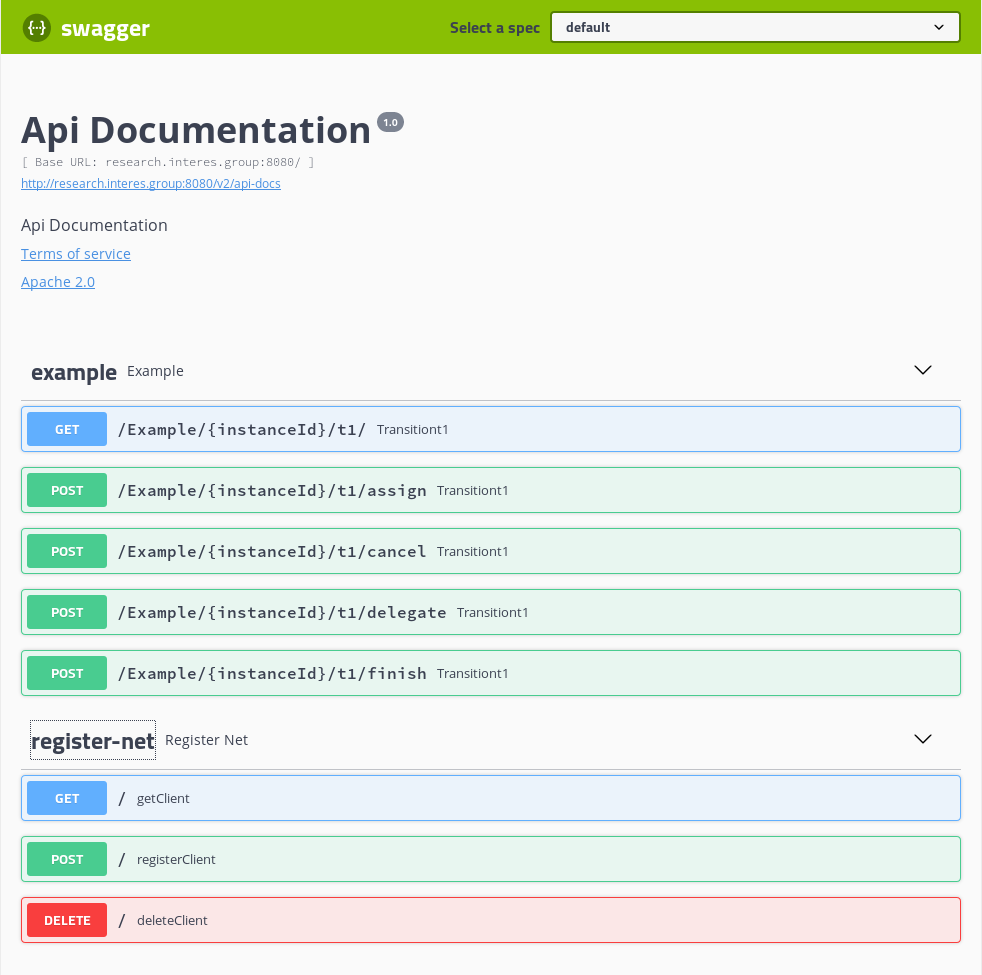
\includegraphics[width=16cm]{img/swagger_ui.png}
	\caption{Ukážka vizualizácie dokumentácie Swagger UI}
	\label{swagger_ui}
\end{figure}

V Swagger UI dokumentácií sa dajú otvoriť jednotlivé koncové body a prezrieť ich detaily. Na obrázku \ref{swagger_ui_endpoint} vidíme príklad detailov koncového bodu finish pre prechod t1. V detailoch vidíme roly, ktoré daný koncový bod môžu použiť, dátové polia, ich typ a či sú povinné. Vidíme tam a aj pole instanceID, ktoré nie je pole z tela dopytu, ale parameter URL.

\begin{figure}[!htbp]
	\centering
	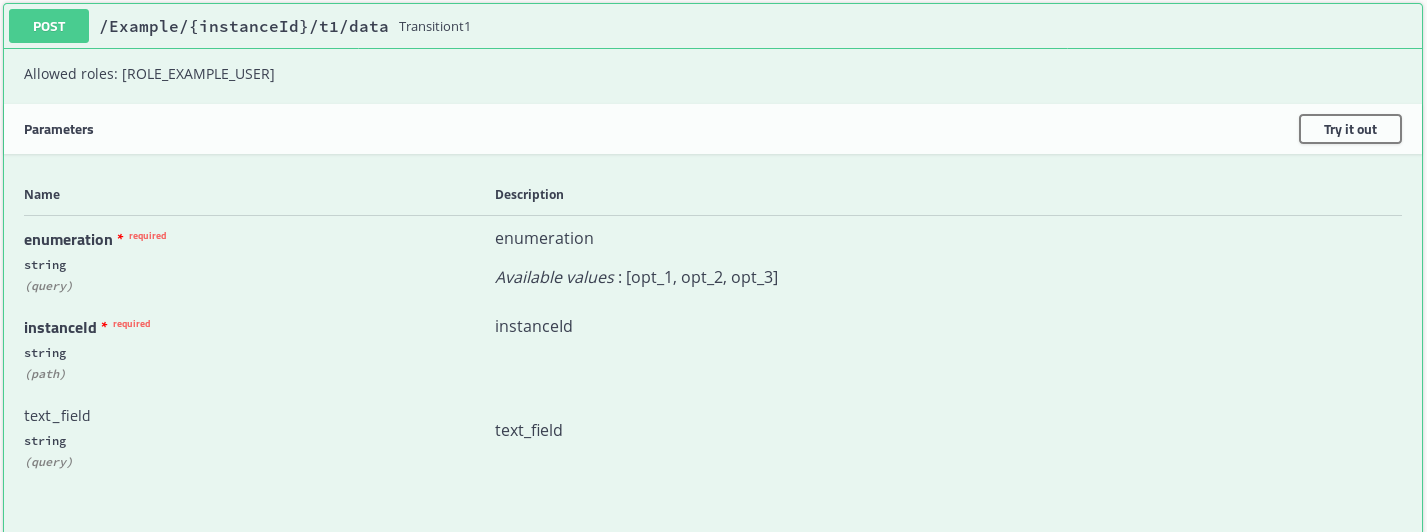
\includegraphics[width=16cm]{img/swagger_ui_endpoint.png}
	\caption{Ukážka vizualizácie dokumentácie kokrétneho koncového bodu}
	\label{swagger_ui_endpoint}
\end{figure}



\subsection{Auth Service}  \label{section_auth}

Na implementáciu autorizačného servera, ktorý dokáže spolupracovať so zvyškom nášho systému sme použili balíček Spring Cloud Security \cite{cloud_security}. Tento balíček podobne ako Spring Boot Security poskytuje základnú funkcionalitu umožňujúcu sa prihlásiť pomocou mena, hesla, alebo aj \acrshort{oauth} a uskladnenie profilov používateľov.

Na rozdiel od základného balíčka Spring Boot Security poskytuje Spring Cloud Security funkcionalitu ktorá umožňuje v centralizovať autentifikáciu do jedného kontajnera. Ostatné kontajnery, ktoré obsahujú koncové body, ktoré chceme zabezpečiť sa označujú ako resource servre.

Resource server, nedrží informácie o používateľoch, ak však príde dopyt na funkciu, ktorá si vyžaduje autorizáciu, vie tento server získať profil používateľa od autorizačného servera. Ak nie je tento používateľ autorizovaný na vykonanie dopytu vracia resource server chybu 403.

Na spustenie autorizačného servera stačí importovať balíky  Spring Cloud Security a Spring Cloud OAuth, napísať základnú konfiguráciu a autorizačný server sa dá spustiť.

Na integráciu so zvyškom nášho systému sme importovali tieto balíky aj do ostatných servisov a v prípade, kedy si funkcionalita vyžiadala autorizáciu  pridali sme potrebné anotácie. Aby sme dosiahli granulárnu kontrolu nad prístupom k funkcionalite, ku každej funkcií sme špecifikovali aké roly k nim majú prístup pomocou príslušnej anotácie.

Pre jednoduchosť implementácie sme na ukladanie profilov používateľov a tokenov využili in memory store. To znamená, že sa pri každom reštarte auth servisu tieto informácie zmažú. Keďže však používame architektúru mikroservisov, a servisy sú od seba do veľkej miery nezávislé, nie je potrebné reštartovať všetky servisy pri zmene jedného. Pri vývoji teda fakt, že používatelia boli uložený vo volatilnej pamäti nebol priveľkou prekážkou. Pre nasadenie systému do produkcie však bude nutné pridať do auth servisu perzistentné úložisko používateľov.

%TODO expand auth service
%TODO auth by classes, by functions

\begin{figure}[!htbp]
	\centering
	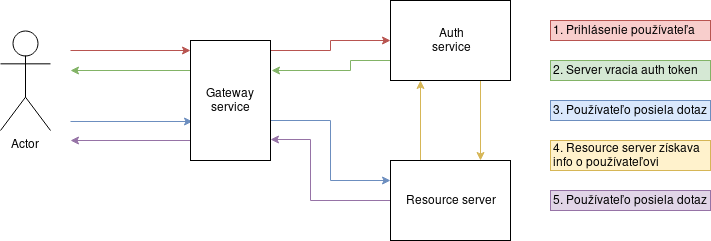
\includegraphics[width=10cm]{img/auth_operation.png}
	\caption{Autorizácia}
	\label{auth_operation}
\end{figure}

\subsection{Service Discovery}
Service discovery je služba ktorá sleduje stav ostatných služieb a vie zabezpečiť koordináciu komunikácie medzi jednotlivými kontajnermi v cloudovom riešení. V našom systéme implementujeme service discovery ako Spring Boot kontajner s balíčkom Netflix Eureka \cite{eureka}. Nastavenie tohto balička si vyžaduje len importovať závislosť, použiť anot @EnableEurekaServer a nastaviť port servera, v našom prípade je to štandardný port 7777 a hostname Eurka servra.

Na to aby sa ostatné kontajnery zahlásili do service discovery sme importovali v nich balíček Netflix Eureka Client, použili anotáciu @EnableDiscoveryClient a nastavili port, na ktorom sa nachádza discovery servis. Na to aby sme vedeli rozlíšiť typ servisu, ktorý sa pripája na service discovery je ešte potrebné zadať do konfigurácie meno servisu.

Na ukážke kódu \ref{alg:eureka_config} vidíme príklad konfigurácie eureka servra a klienta.

\begin{lstlisting}[float, caption={Konfigurácia Eureka servra a klienta},label={alg:eureka_config},language=yaml]
# Eureka server
server:
  port: 7777
  eureka:
	instance:
	  hostname: localhost
			

# Discovery client	
spring:
  application:
	name: generator-service
eureka:
  client:
	serviceUrl:
	  defaultZone: "http://localhost:7777/eureka"
\end{lstlisting}

Po správnej inicializácií servera a klientov je na porte 7777 dostupná stránka s grafickým rozhraním. Na obrázku \ref{eureka_gui} vidíme screenshoot tejto obrazovky v našom testovacom prostredí. na obrázku vidíme základné informácie o serveri a tabuľku so zaregistrovanými kontajnermi nášho rozhrania. Vidíme, že na porte 8088 beží auth servis, na porte 8080 beží gateway, na porte 8081 beží generátor a na portoch 8082-8085 bežia štyri inštancie relay servisu.

\begin{figure}[!htbp]
	\centering
	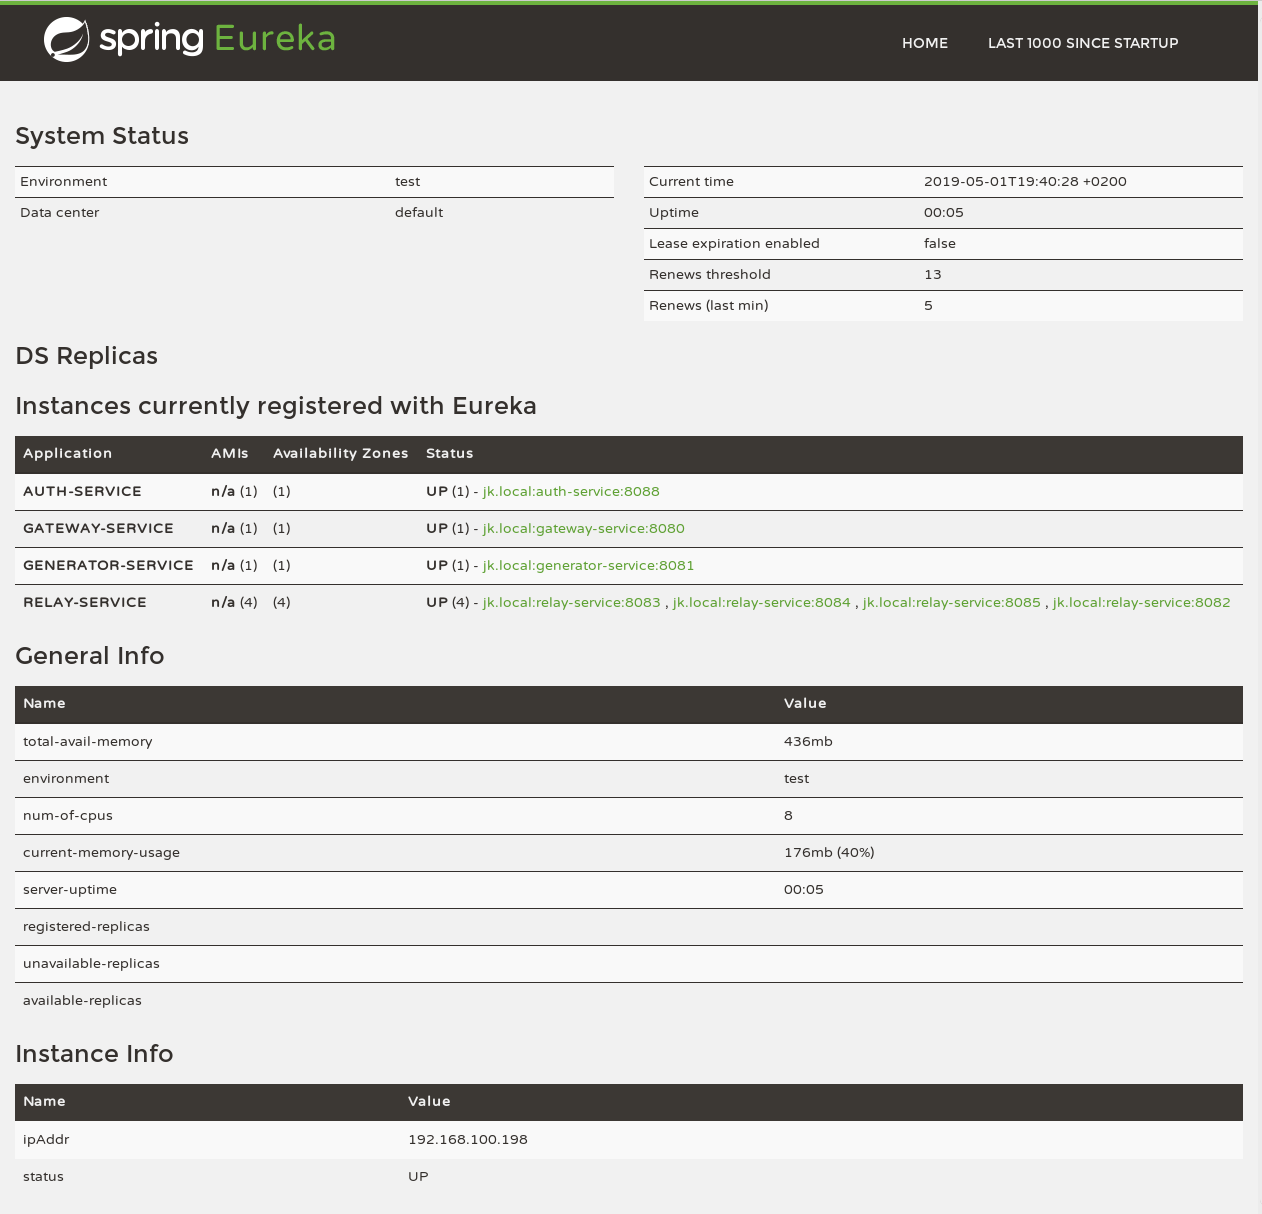
\includegraphics[width=16cm]{img/eureka_gui.png}
	\caption{Užívateľské rozhranie Spring Eureka}
	\label{eureka_gui}
\end{figure}

\subsection{Gateway Service}
Gateway service je rovnako ako ostatné servisy implementovaný ako Spring Boot aplikácia s pridaným balíkom Spring Cloud Gateway \cite{cloud_gateway}, ktorý zabezpečuje funkcionalitu routingu a load balancera.
Na spustenie základnej funkcionality routingu v tomto prípade netreba použiť žiadnu anotáciu, stačí len zadefinovať trasy a k nim prislúchajúce filtre. Na ukážke kódu \ref{alg:gateway_config} vidíme konfiguráciu nášho gateway servisu. Na začiatku je definovaný port na ktorom počúva server, tento port je jediný port, ktorý bude prístupný vonkajšiemu svetu.

\begin{lstlisting}[float, caption={Konfigurácia Gateway servisu},label={alg:gateway_config},language=yaml]
server:
  port: 8080
eureka:
  client:
    serviceUrl:
      defaultZone: http://localhost:7777/eureka/
spring:
  application:
    name: gateway-service
  cloud:
    gateway:
      discovery:
        locator:
          enabled: true
          lower-case-service-id: true
      routes:
        - id: register_route
          uri: "http://localhost:8081/"
          predicates:
            - "Path=/"
        - id: auth_route
          uri: "http://localhost:8088/oauth/"
          predicates:
            - "Path=/oauth/**"
        - id: get_user_route
          uri: "http://localhost:8088/user"
          predicates:
            - "Path=/user"
        - id: endoint_route
          uri: "lb://RELAY-SERVICE/"
          predicates:
            - "Path=/**"
\end{lstlisting}

Prvá \acrshort{url} ktorú máme v konfigurácií zadefinovanú je "/". Táto \acrshort{url} obsahuje funkcie obsluhu nášho rozhrania táto URL je smerovaná na generator service na porte 8081.
Nasledujúce dve trasy smerujú na Auth servis na porte 8088. Prvá obsluhuje dopyty na autentifikáciu cez \acrshort{oauth}, druhá smeruje dopyt na získanie informácií o aktuálnom používateľovi.

Posledná trasa smeruje všetky ostatné dopyty na relay servis. Ako môžeme vidieť URI cieľovej služby nie je s protokolom HTTP a portom na ktorom je služba a ale s protokolom lb a menom služby. Takáto notácia nám umožňuje využiť load balancer balíka Spring Cloud Gateway. Na to aby sme mohli využívať tento protokol musíme ešte nakonfigurovať spojenie so službou service discovery. Ak povolíme možnosť discovery locator, náš gateway servis si vypýta od service discovery informácie o lokácií služieb v našom cloudovom riešení a následne sme schopní adresovať ich pomocou mena, namiesto URI, a môžeme využívať možnosti load balancera. Load balancer sa dá nastaviť aj aby so statickým zoznamom URI jednotlivých inštancii služieb, riešenie cez service discovery locator sa však ukázalo ako praktickejšie, keďže vie dynamicky reagovať na počet spustených inštancií.

Na operáciu gateway servisu nepotrebujeme žiadnu ďalšiu konfiguráciu. Všetky dopyty sú správne smerované servisom, pre ktoré sú určené.

\subsection{Platforma}
%todo rename?
V nasledujúcej časti si priblížime aké prostredie sme využívali na vývoj a testovanie systému, ďalej si popíšeme kroky, ktoré sú potrebné na spustenie našej aplikácie

Platforma na ktorú sme nasadzovali náš systém je virtuálny server poskytnutý Fakultou Elektrotechniky a Informatiky na Slovenskej Technickej Univerzite v Bratislave s operačným systémom Ubuntu 18.04.2 LTS Bionic Beaver. Server má k dispozícií 10GB operačnej pamäte, 4GB swap, a 8 jadier procesora.

Pred tým ako sa pokúsime spustiť systém treba sa uistiť, že server, na ktorý plánujeme systém nasadiť bude mať aspoň 8GB voľnej operačnej pamäte a aspoň 2 procesorové jadrá.
Na nasadenie našej aplikácie potrebujeme vykonať nasledovné kroky:

\begin{enumerate}
    \item Uistíme sa, že na serveri je nainštalovaný nástroj Git a Java 8.
	\item Pomocou gitu stiahneme repozitár \cite{dp_repo} s aktuálnou verziou nášho systému.
    \item Skompilujeme a spustíme programu pomocou skriptu "run.sh" ktorý sa nachádza v priečinku repozitára. Tento skript stiahne Gradle 5.4.1, A postupne nainštaluje a spustí všetky kontajnery nášho systému.
	Proces kompilácie a spúšťania kontajnerov je výpočtovo náročný a na serveroch so štyrmi a menej jadrami môže trvať viac ako 3 minúty. Pri prvom spustení si bude inštalačný skript sťahovať závislosti, preto tento proces môže trvať ešte dlhšie.
    \item Povolíme prístup na port 8080 z internetu. 8080 je prednastavený port, na ktorom počúva naša aplikácia. Ak port 8080 nie je vyhovujúci dá sa nastaviť v súbore /gateway/src/resources/application.yml zmenením hodnoty server.port
    \item Na porte 7777 je prezentovane grafické rozhranie service discovery, tento port z bezpečnostných dôvodov neodporúčame povoliť cez firewall, namiesto toho na monitorovanie stavu systému odporúčame použiť ssh tunel pre tento port.
\end{enumerate}

\section{Testovanie}
V tejto kapitole si priblížime proces testovania ktorý sme využívali pri vývoji systému a systém automatizovaného testovania, ktorý sme implementovali na systéme.

\subsection{Manuálne testy}

Na manuálne testovanie počas vývoja sme používali softvér Insomnia REST Client\cite{insomnia}. V tomto programe sme vytvorili rôzne volania na náš systém a kontrolovali sme ich výstup.

\subsubsection{Auth service}
Pri autorizačnom serveri sme testovali, či základným systémovým používateľom bude správne pridelený autorizačný token a či tento token je platný. Na obrázku \ref{insomnia_oauth} vidíme príklad takéhoto dopytu. Na príklade vidíme, že po vyplnení správnych údajov do karty OAuth 2 v programe Insomnia môžeme odoslať dopyt na zabezpečený koncový bod v našej aplikácií a dopyt vráti správnu odpoveď.
\begin{figure}[!htbp]
	\centering
	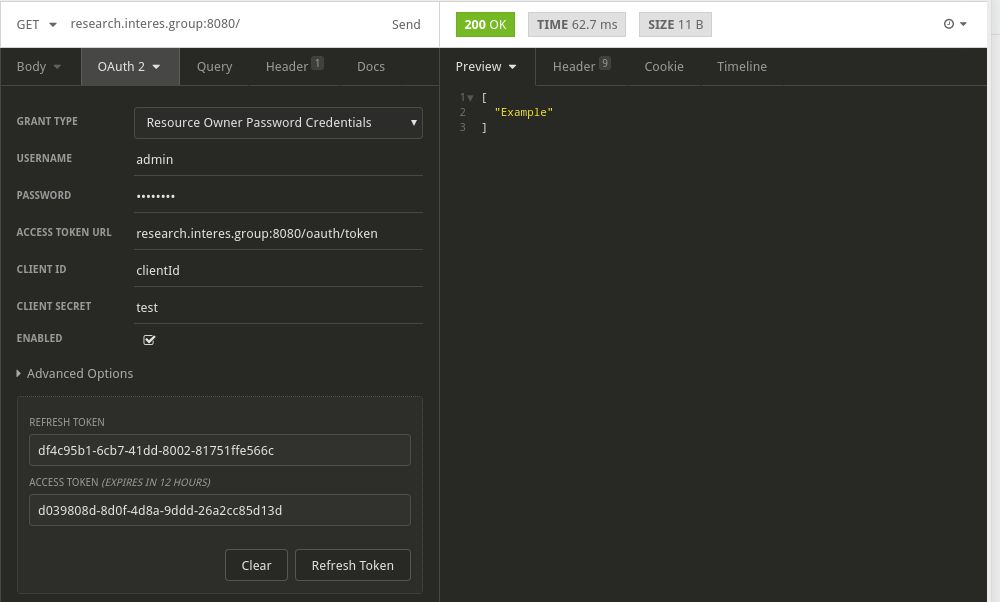
\includegraphics[width=16cm]{img/insomnia_oauth.png}
	\caption{Ukážka testu auth servisu}
	\label{insomnia_oauth}
\end{figure}

\subsubsection{Gateway service}
Pri gateway service sme testovali správne nastavenie smerovania, a či server naozaj smeruje dotazy na správny server. Ďalej sme testovali funkcionalitu load balancera. Tú sme testovali tak, že sme spustili viaceré inštancie relay servisu, s miernymi zmenami v kóde a load balancer naše dopyty smeroval striedavo na rôzne inštancie relay servisu.

\subsubsection{Generator service}
Pri generator service sme testovali či sa vygeneroval spustiteľný kód. V prípade, že kód ktorý sa vygeneroval nebol syntakticky správny vrátil koncový bod generátora chybovú odpoveď. Jedna z chýb ktoré sme pri takomto testovaní objavili je chyba knižnice kotlinpoet, kedy sa pri generovaní zalomí dlhší text bez ošetrenia úvodzoviek a teda sa vygeneruje nevalidný kód.

Ak sa korektne vygeneroval kód a spustila sa nová inštancia relay servisu testovali sme, či vygenerovaný kód validácie funguje korektne.

Ďalej sme pri tejto službe testovali, či sa pri regenerácií relay servisu prejavila zmena v dokumentácií korektne, a či sa správne zaregistrovali používatelia v auth servise.

\subsubsection{Relay service}
Pri tomto servise sme testovali funkčnosť validačných funkcií. Testovali sme, či neprítomnosť povinného dátového poľa vráti správnu chybovú hlášku, a či pri poliach s predpísaným formátom vstupu vráti servis chybu ak formát vstupu nie je korektný a či ak je formát správny prebehne funkcia korektne a vráti pozitívny výsledok. Na obrázku \ref{insomnia_200} vidíme príklad korektného dotazu a na obrázku \ref{insomnia_400} vidíme príklad dopytu, ktorý nemá správny formát dát v poli s enumeráciou.

\begin{figure}[!htbp]
	\centering
	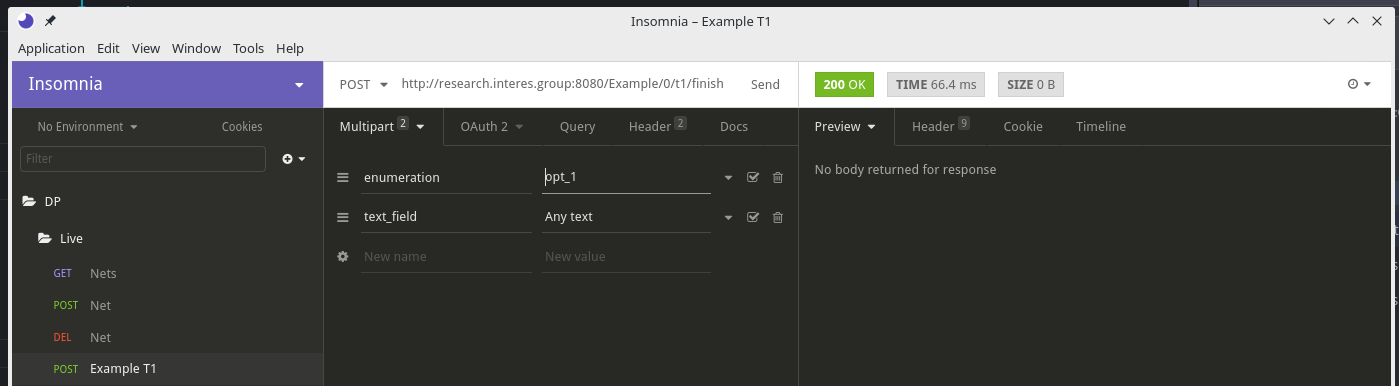
\includegraphics[width=16cm]{img/insomnia_200.png}
    \caption{Ukážka vizualizácie dokumentácie konkrétneho koncového bodu}
	\label{insomnia_200}
\end{figure}

\begin{figure}[!htbp]
	\centering
	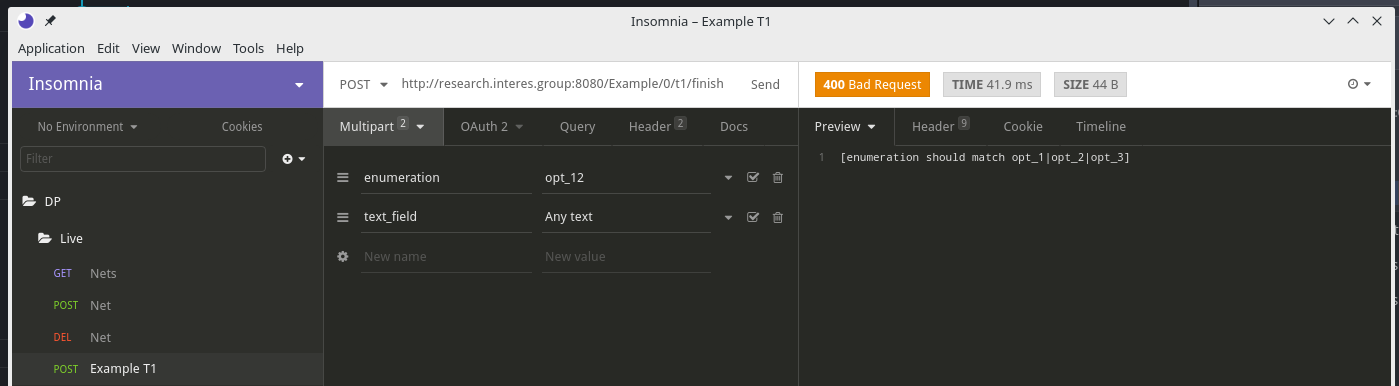
\includegraphics[width=16cm]{img/insomnia_400.png}
    \caption{Ukážka vizualizácie dokumentácie konkrétneho koncového bodu}
	\label{insomnia_400}
\end{figure}

\subsection{Automatizované testy}

%TODO auto test relay service
